% Problem 11
\Needspace{18\baselineskip}
\item \label{prob:11}
\noindent\begin{minipage}[t]{0.6\linewidth}
\vspace{0pt}
A piece of an ideal fluid is marked as it moves along a horizontal streamline through a pipe, as shown in the figure. In Region I, the speed of the fluid on the streamline is $V$. The cylindrical, horizontal pipe narrows so that the radius of the pipe in Region II is half of what it was in Region I. What is the speed of the marked fluid when it is in Region II?
\begin{enumerate}[label=(\Alph*)]
    \item 4$V$
    \item 2$V$
    \item $V$
    \item $V/2$
    \item $V/4$
\end{enumerate}
\end{minipage}%
\hfill
\begin{minipage}[t]{0.35\linewidth}
\vspace{0pt}
\centering
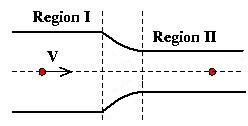
\includegraphics[width=\linewidth]{Problem_11_Figure.png}
\end{minipage}

\category{Fluid Mechanics}
\StudyGuideLinks{11}
\ProblemSource{11} 
\begin{answerbox}
\finalanswer{(A) 4V}
\end{answerbox}
\begin{insightbox}
Continuity $A_1v_1=A_2v_2$: halving the radius quarters the area, so the speed quadruples.
\end{insightbox}
\begin{solutionbox}

Continuity: $A_1 v_1 = A_2 v_2$ with $A\propto r^2$. If $r_2=\tfrac{1}{2}r_1$, then $A_2=\tfrac{1}{4}A_1$, so $v_2 = (A_1/A_2) v_1 = 4V$.
\end{solutionbox}

% Problem 12
\Needspace{18\baselineskip}
\item \label{prob:12}
\noindent\begin{minipage}[t]{0.6\linewidth}
\vspace{0pt}
For the RC circuit shown, the resistance is $R = 10.0 \Omega$, the capacitance is $C = 5.0\,\mathrm{F}$ and the battery has voltage $\mathcal E = 12$ volts. The capacitor is initially uncharged when the switch S is closed at time $t = 0$. At some time later, the current in the circuit is $0.50$ A. What is the magnitude of the voltage across the capacitor at that moment?
\begin{enumerate}[label=(\Alph*)]
    \item 0 volts
    \item 5 volts
    \item 6 volts
    \item 7 volts
    \item 12 volts
\end{enumerate}
\end{minipage}%
\hfill
\begin{minipage}[t]{0.35\linewidth}
\vspace{0pt}
\centering
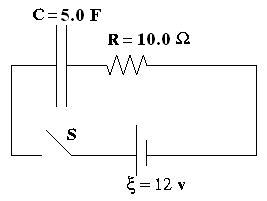
\includegraphics[width=\linewidth]{Problem_12_Figure.png}
\end{minipage}

\category{RC Circuits}
\StudyGuideLinks{12}
\ProblemSource{12}
\begin{answerbox}
\finalanswer{(D) 7 volts}
\end{answerbox}
\begin{insightbox}
KVL: $\mathcal E=V_R+V_C$. With $I$ known, find $V_R=IR$ then $V_C$.
\end{insightbox}
\begin{solutionbox}

KVL: $\mathcal E - V_R - V_C = 0$. With $I=0.50\,\text{A}$ and $R=10.0\,\Omega$, $V_R=IR=5.0\,\text{V}$. Hence $V_C=\mathcal E - V_R = 12-5=7\,\text{V}$.
\end{solutionbox}

% Problem 13
\Needspace{18\baselineskip}
\item \label{prob:13}
A ball initially at rest falls without air resistance from a height $h$ above the ground. If the ball falls the first distance $h/2$ in a time $t$, how much time is required to fall the remaining distance of $h/2$?
\begin{enumerate}[label=(\Alph*)]
    \item 0.25$t$
    \item 0.41$t$
    \item 0.50$t$
    \item 0.71$t$
    \item 1.00$t$
\end{enumerate}

\category{Kinematics}
\StudyGuideLinks{13}
\ProblemSource{13}
\begin{answerbox}
\finalanswer{(B) 0.41t}
\end{answerbox}
\begin{insightbox}
First half gives $h=gt^2$; total time is $\sqrt2 t$, so the remainder is $(\sqrt2-1)t\approx0.414t$.
\end{insightbox}
\begin{solutionbox}

With $d=\tfrac{1}{2}gt^2$, first half: $h/2=\tfrac{1}{2}gt^2\Rightarrow h=gt^2$. Total time $t_{\text{tot}}$ satisfies $h=\tfrac{1}{2}g t_{\text{tot}}^2\Rightarrow t_{\text{tot}}=\sqrt{2}t$. Remaining time $t_{\text{rem}}=t_{\text{tot}}-t=(\sqrt{2}-1)t\approx 0.414t$.
\end{solutionbox}

% Problem 14
\Needspace{18\baselineskip}
\item \label{prob:14}
\noindent\begin{minipage}[t]{0.6\linewidth}
\vspace{0pt}
An object of mass M starts from rest at the bottom of a fixed incline of height H. A person decides to push the object up the incline in one of two ways with an applied force shown in the diagram. In each of the trials, the object reaches the top of the incline with speed $V$. How would the work done by the person on the block compare for the two trials? Assume the same constant non-zero coefficient of kinetic friction.
\begin{enumerate}[label=(\Alph*)]
    \item More work would be done in Trial 1
    \item More work would be done in Trial 2
    \item The work would be equal for both trials
    \item Impossible to determine without knowing $V$.
    \item Impossible to determine without knowing $\mu_k$.
\end{enumerate}
\end{minipage}%
\hfill
\begin{minipage}[t]{0.35\linewidth}
\vspace{0pt}
\centering
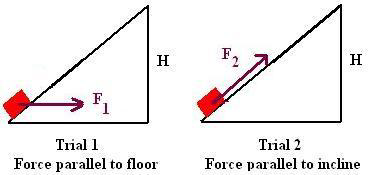
\includegraphics[width=\linewidth]{Problem_14_Figure.png}
\end{minipage}

\category{Work \& Energy with Friction}
\StudyGuideLinks{14}
\ProblemSource{14} 
\begin{answerbox}
\finalanswer{(A) More work would be done in Trial 1}
\end{answerbox}
\begin{insightbox}
A horizontal push raises the normal force and friction loss; since $\Delta K$ and $W_g$ match, external work must be larger.
\end{insightbox}
\begin{solutionbox}

Horizontal push increases the normal force: $N_1=Mg\cos\theta+F_1\sin\theta>Mg\cos\theta=N_2$, so friction is larger in Trial 1. Since $\Delta K$ and $W_g$ are the same, the greater friction loss requires more input work in Trial 1.
\end{solutionbox}

% Problem 15
\Needspace{18\baselineskip}
\item \label{prob:15}
\noindent\begin{minipage}[t]{0.6\linewidth}
\vspace{0pt}
A point object with mass $M=2.0$kg is attached a distance $R=1.75$m from the fixed center of a disk. The disk starts rotating from rest with constant angular acceleration $\alpha = 5.00$ rad/s$^2$. After how much time $T$ (in seconds) is the tangential acceleration equal in magnitude to the centripetal acceleration?
\begin{enumerate}[label=(\Alph*)]
    \item 0.769
    \item 0.592
    \item 0.500
    \item 0.447
    \item 0.350
\end{enumerate}
\end{minipage}%
\hfill
\begin{minipage}[t]{0.35\linewidth}
\vspace{0pt}
\centering
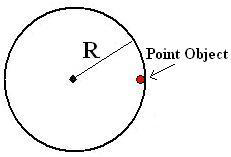
\includegraphics[width=\linewidth]{Problem_15_Figure.png}
\end{minipage}

\category{Rotational Kinematics}
\StudyGuideLinks{15}
\ProblemSource{15} 
\begin{answerbox}
\finalanswer{(D) 0.447}
\end{answerbox}
\begin{insightbox}
Set $a_t=R\alpha$ equal to $a_c=R(\alpha T)^2$ to get $T=1/\sqrt{\alpha}$.
\end{insightbox}
\begin{solutionbox}

Set $a_t=R\alpha$ equal to $a_c=R\omega^2=R(\alpha T)^2$. Then $R\alpha=R\alpha^2 T^2\Rightarrow T=1/\sqrt{\alpha}=1/\sqrt{5}\approx0.447\,\text{s}$.
\end{solutionbox}

% Problem 16
\Needspace{18\baselineskip}
\item \label{prob:16}
\noindent\begin{minipage}[t]{0.6\linewidth}
\vspace{0pt}
A uniform, solid cylinder with a mass M and radius R is pulled by a horizontal force F acting through the center as shown. The cylinder rolls to the right without slipping. What is the magnitude of the force of friction between the cylinder and the ground?
\begin{enumerate}[label=(\Alph*)]
    \item $\frac{1}{4}F$
    \item $\frac{1}{3}F$
    \item $\frac{1}{2}F$
    \item $\frac{2}{3}F$
    \item $\frac{3}{4}F$
\end{enumerate}
\end{minipage}%
\hfill
\begin{minipage}[t]{0.35\linewidth}
\vspace{0pt}
\centering
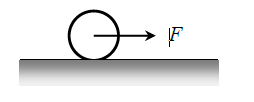
\includegraphics[width=\linewidth]{Problem_16_Figure.png}
\end{minipage}

\category{Rolling Dynamics}
\StudyGuideLinks{16}
\ProblemSource{16} 
\begin{answerbox}
\finalanswer{(B) $\tfrac{1}{3}F$}
\end{answerbox}
\begin{insightbox}
Combine translation $F-f=Ma$ with rotation $fR=I\alpha$ and $a=R\alpha$ to obtain $f=F/3$.
\end{insightbox}
\begin{solutionbox}

Translational: $F-f=Ma$. Rotational: $fR=I\alpha$ with $I=\tfrac{1}{2}MR^2$ and $a=R\alpha$. Then $f=\tfrac{1}{2}Ma$. Sub into translation: $F-f=2f\Rightarrow F=3f\Rightarrow f=F/3$.
\end{solutionbox}

% Problem 17
\Needspace{18\baselineskip}
\item \label{prob:17}
A comet moves in an elliptical orbit around the sun. As the comet moves from aphelion (farthest point) to perihelion (closest point), which of the following results is true?
\begin{enumerate}[label=(\Alph*)]
    \item Speed of the comet: Increases, Angular momentum of the comet/sun system: Increases, Gravitational potential energy of the comet/sun system: Decreases
    \item Speed of the comet: Increases, Angular momentum of the comet/sun system: Constant, Gravitational potential energy of the comet/sun system: Decreases
    \item Speed of the comet: Decreases, Angular momentum of the comet/sun system: Decreases, Gravitational potential energy of the comet/sun system: Increases
    \item Speed of the comet: Increases, Angular momentum of the comet/sun system: Increases, Gravitational potential energy of the comet/sun system: Constant
    \item Speed of the comet: Constant, Angular momentum of the comet/sun system: Constant, Gravitational potential energy of the comet/sun system: Constant
\end{enumerate}

\category{Gravitation}
\StudyGuideLinks{17}
\ProblemSource{17} 
\begin{answerbox}
\finalanswer{(B) Increases, Constant, Decreases}
\end{answerbox}
\begin{insightbox}
Zero torque about the sun conserves angular momentum; as $r$ decreases, $U=-GMm/r$ drops and speed rises.
\end{insightbox}
\begin{solutionbox}

Central gravity gives zero torque, so angular momentum is conserved. As $r$ decreases, $U=-GMm/r$ decreases, hence kinetic energy and speed increase.
\end{solutionbox}

% Problem 18
\Needspace{18\baselineskip}
\item \label{prob:18}
\noindent\begin{minipage}[t]{0.6\linewidth}
\vspace{0pt}
An open cylindrical container with very large radius is at rest a distance $H$ above the ground at the edge of a platform. A tiny hole develops at the bottom of the container and water from the container squirts out horizontally landing a distance $H$ from the edge of the platform. For the water to land at this location, what is the depth of the water $L$ in the container? The figure is not drawn to scale and air resistance is ignored.
\begin{enumerate}[label=(\Alph*)]
    \item $H/4$
    \item $H/\sqrt{2}$
    \item $H$
    \item $H\sqrt{2}$
    \item $2H$
\end{enumerate}
\end{minipage}%
\hfill
\begin{minipage}[t]{0.32\linewidth}
\vspace{0pt}
\centering
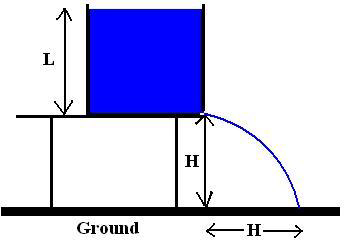
\includegraphics[width=\linewidth]{Problem_18_Figure.png}
\end{minipage}

\category{Fluid Mechanics \& Projectile Motion}
\StudyGuideLinks{18}
\ProblemSource{18} 
\begin{answerbox}
\finalanswer{(A) $H/4$}
\end{answerbox}
\begin{insightbox}
Torricelli gives $v=\sqrt{2gL}$; range $H$ equals $v$ times fall time $\sqrt{2H/g}$.
\end{insightbox}
\begin{solutionbox}

Torricelli: $v=\sqrt{2gL}$. Time of fall from height $H$ is $t=\sqrt{2H/g}$. Range $H=v t=\sqrt{2gL}\,\sqrt{2H/g}=\sqrt{4LH}$. Hence $H^2=4LH\Rightarrow L=H/4$.
\end{solutionbox}

% Problem 19
\Needspace{18\baselineskip}
\item \label{prob:19}
\noindent\begin{minipage}[t]{0.6\linewidth}
\vspace{0pt}
A monatomic ideal gas is the working substance for an engine that undergoes the cyclic process (ABCDA) shown in the PV diagram. The processes are all isochoric or isobaric with pressures between $P_0$ and $2P_0$ and volumes between $V_0$ and $\frac{3}{2}V_0$. What is the efficiency of this engine?
\begin{enumerate}[label=(\Alph*)]
    \item $1/8$
    \item $1/5$
    \item $1/3$
    \item $2/3$
    \item $5/7$
\end{enumerate}
\end{minipage}%
\hfill
\begin{minipage}[t]{0.32\linewidth}
\vspace{0pt}
\centering
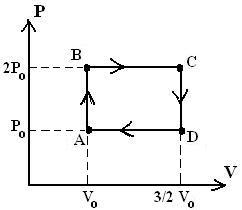
\includegraphics[width=\linewidth]{Problem_19_Figure.png}
\end{minipage}

\category{Thermodynamics \& Engines}
\StudyGuideLinks{19}
\ProblemSource{19} 
\begin{answerbox}
\finalanswer{(A) 1/8}
\end{answerbox}
\begin{insightbox}
Compute heat on isobaric/isochoric legs; net work is rectangle area $\Delta P\,\Delta V$; efficiency is $W/Q_{in}$. Sign guide: isobaric expansion (heat in, $W>0$), isochoric heating (heat in, $W=0$), isobaric compression (heat out, $W<0$), isochoric cooling (heat out, $W=0$).
\end{insightbox}
\begin{solutionbox}

Net work: $W=\Delta P\,\Delta V= (2P_0-P_0)\,(\tfrac{3}{2}V_0-V_0)=\tfrac{1}{2}P_0V_0$. Heat in during AB and BC: $Q_{in}=\tfrac{3}{2}P_0V_0+\tfrac{5}{2}P_0V_0=4P_0V_0$. Efficiency $\eta=W/Q_{in}=1/8$.
\end{solutionbox}

% Problem 20
\Needspace{18\baselineskip}
\item \label{prob:20}
\noindent\begin{minipage}[t]{0.6\linewidth}
\vspace{0pt}
A solid, uniform sphere rolls without slipping on a floor along the +x-axis. The rotational kinetic energy associated with the sphere about an axis through its center of mass along the +z-axis is 20 Joules. What is the translational kinetic energy associated with the sphere?
\begin{enumerate}[label=(\Alph*)]
    \item 8 J
    \item 10 J
    \item 20 J
    \item 40 J
    \item 50 J
\end{enumerate}
\end{minipage}%
\hfill
\begin{minipage}[t]{0.32\linewidth}
\vspace{0pt}
\centering
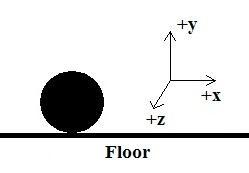
\includegraphics[width=\linewidth]{Problem_20_Figure.png}
\end{minipage}

\category{Rolling Energy}
\StudyGuideLinks{20}
\ProblemSource{20} 
\begin{answerbox}
\finalanswer{(E) 50 J}
\end{answerbox}
\begin{insightbox}
With pure rolling $v=R\omega$, a solid sphere has $K_{rot}=\tfrac{1}{5}mv^2$, so $K_{trans}=(5/2)K_{rot}$.
\end{insightbox}
\begin{solutionbox}

For a solid sphere, $I=\tfrac{2}{5}mR^2$ and $v=R\omega$. Then $K_{rot}=\tfrac{1}{2}I\omega^2=\tfrac{1}{5}mv^2$. Meanwhile $K_{trans}=\tfrac{1}{2}mv^2=\tfrac{5}{2}K_{rot}=50\,\text{J}$.
\end{solutionbox}
